
%(BEGIN_QUESTION)
% Copyright 2011, Tony R. Kuphaldt, released under the Creative Commons Attribution License (v 1.0)
% This means you may do almost anything with this work of mine, so long as you give me proper credit

This level-control system is supposed to maintain a constant liquid level inside the knockout drum, preventing liquid from entering the compressor as well as gas from entering the scavenging pump.  Yet, for some reason liquid did manage to enter the compressor, causing the compressor to violently fail:

$$\includegraphics[width=15.5cm]{i00701x01.eps}$$

A trend recording of liquid level and control valve position captured before the explosion holds the only clue as to why this happened.  Examine it to see if you can determine the source of the trouble:

$$\includegraphics[width=15.5cm]{i00701x02.eps}$$

\vfil 

\underbar{file i00701}
\eject
%(END_QUESTION)





%(BEGIN_ANSWER)

This is a graded question -- no answers or hints given!

%(END_ANSWER)





%(BEGIN_NOTES)

We know that liquids are incompressible, and thus the introduction of liquid into a compressor is a likely cause of catastrophic failure.  The trend shows the knock-out drum's level rapidly rising prior to the incident, giving further evidence of liquid intrusion as the cause of compressor failure.

\vskip 10pt

The fact that the trend shows the controller output ramping up rapidly as the level rises tells us the controller was in automatic mode, and that it was trying to do the right thing: the control valve should have been opening up to let more liquid out of the knock-out drum.  The fact that liquid level kept rising despite the controller's valiant effort suggests a problem somewhere in the output of this level control system.

\vskip 10pt

Most likely, the control valve failed shut, probably caused by a lack of instrument air signal.  Meanwhile, the transmitter registered the increasing level, and the controller tried to reverse this trend by driving the output signal up to saturation very rapidly.

Another possible cause for this incident is a manual block valve downstream of the control valve being shut off.  Yet another possibility is the scavenging pump turning off.  Anything that would prevent liquid from leaving the knock-out drum despite an increasing signal to open the control valve could account for what happened.

%INDEX% Process troubleshooting: diagnosing problem via trend recording

%(END_NOTES)


